\section{Results from test runs}
\label{sec:resul}
All the results shown below are derived by running FjordOs CL on the computer Vilje at the Norwegian High Performance facilities. We show results from a 
\begin{itemize}
	\item A hindcast initialized from NorKyst800 on April 1, 2014 and continued up to and including the month of December 2015, and 
	\item Test forecast runs from 2015 (lead time 48 hours). 
\end{itemize}
All inputs are as described in Section \ref{subsec:atmos}.
 
The results from the hindcast are further discussed and evaluated in some detail in an upcoming report \citep{hjelm:etal:2016}. Here we merely present snapshots of fields of currents, temperature, salinity and sea level so as to properly appreciate the level of details that the FjordOs CL model provides. In this we focus on six areas, namely the Inner Oslofjord, the Drammensfjord, the {\DR} area (henceforth {\DR}), the mid part of the Oslofjord (henceforth Slagen), the outer western part (henceforth Tristein) and the outer eastern part of the Oslofjord (henceforth Hvaler). 

\subsection{Hindcast results}

\subsubsection{Currents}
 Figures of interest 

\subsubsection{Temperature}
Figures of interest 

\subsubsection{Salinity}
Figures of interest 

\subsubsection{Sea level}
Figures of interest 

\subsection{Forecast results}

\subsubsection{Currents}
Figures of interest 
%%%%%%%%%%%%%%%%%%% Figure 2 Bathymetry and currents in the Drøbak area %%%%%%%%%%%%%%%
\begin{figure}[t]
  \begin{pspicture}(0,0)(15,12)
% Include graphs
	\rput[b](7.5,0){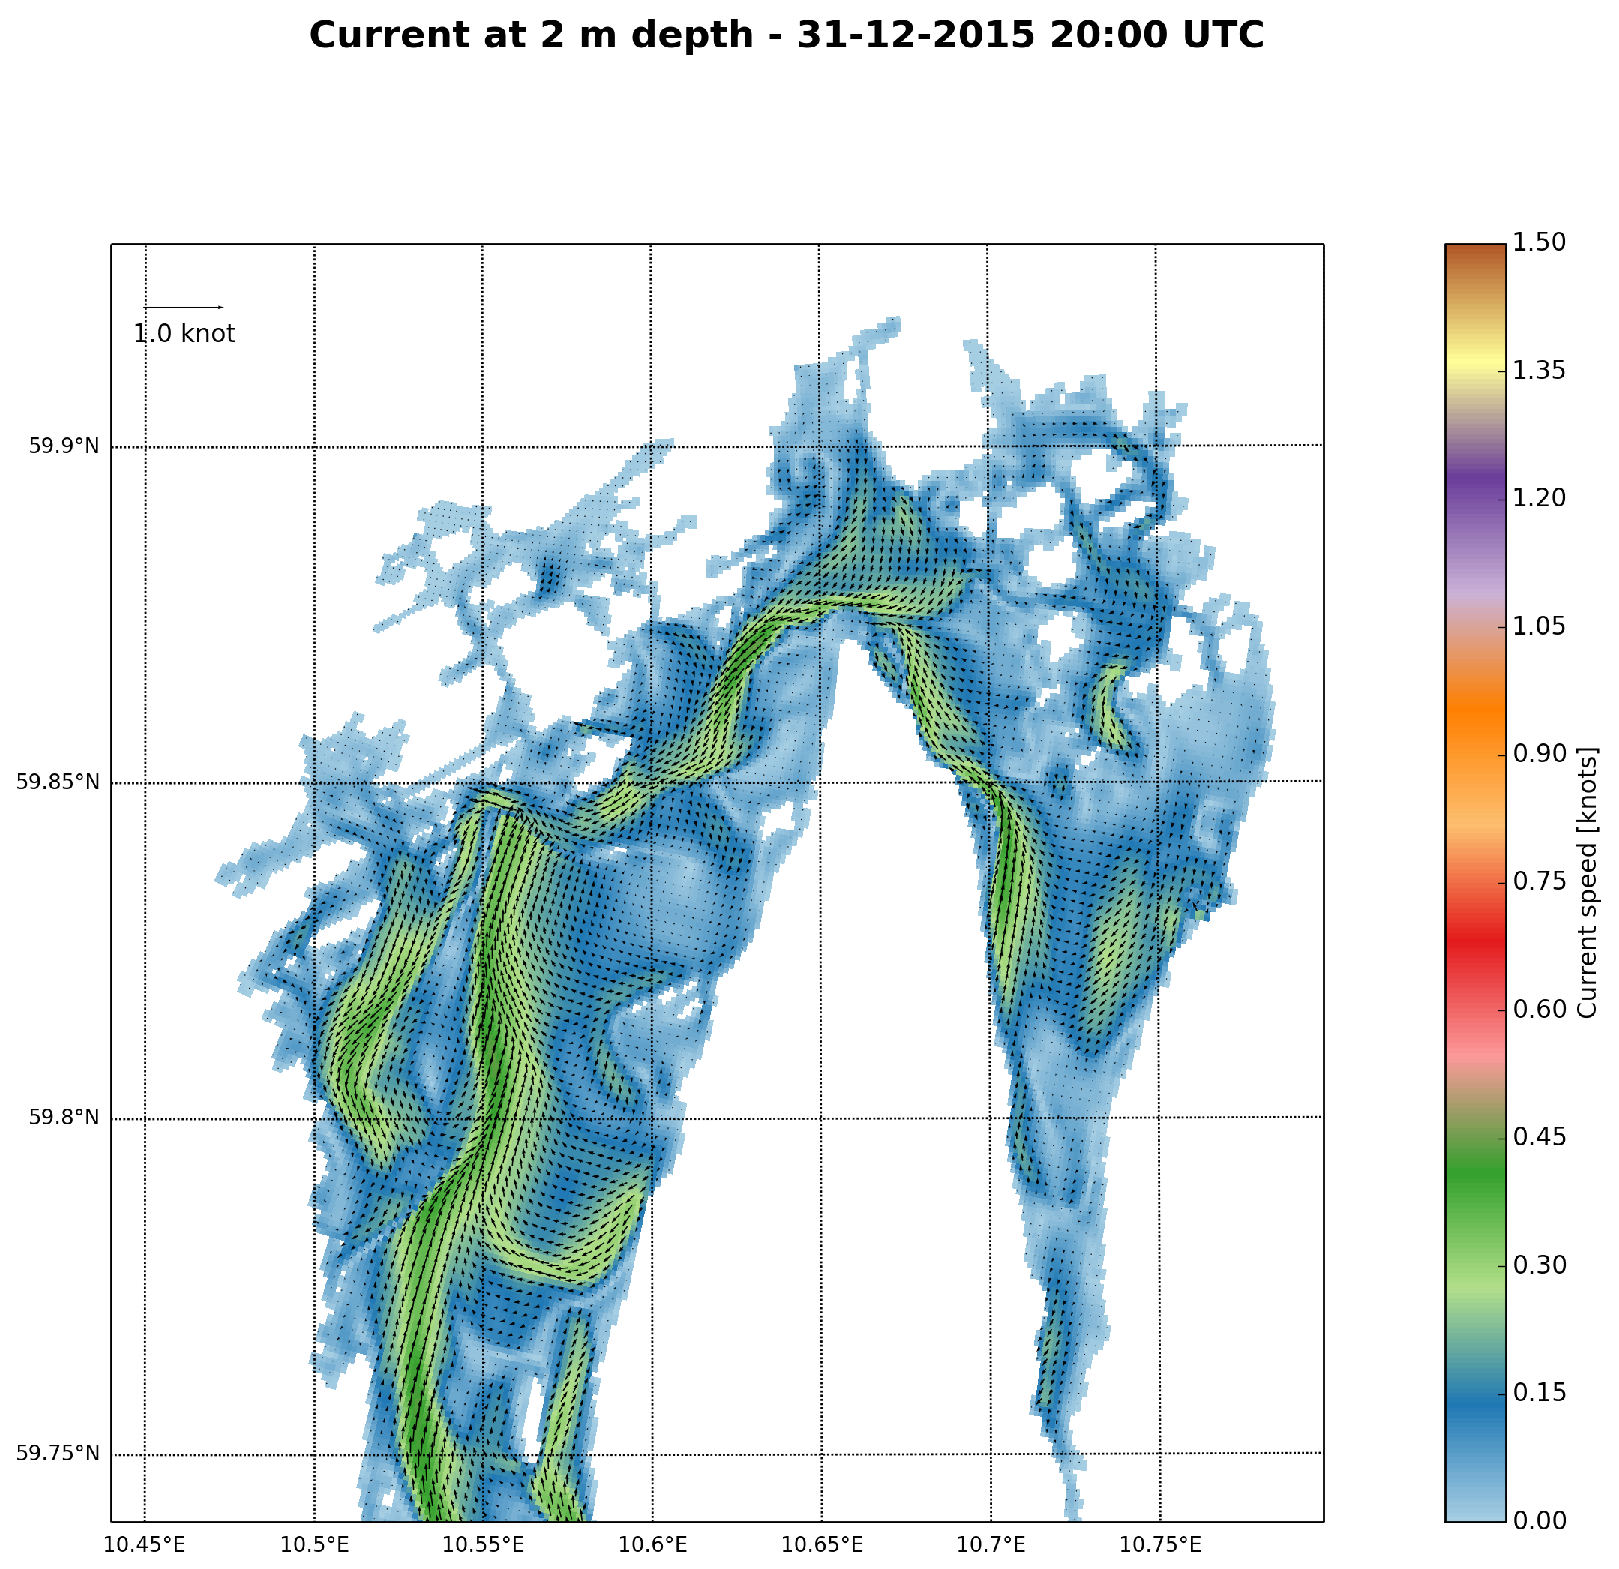
\includegraphics[height=12cm]{indre__56_current}}
  \end{pspicture}
  \caption{\small Forecasted currents at 2 m depth in the inner part of the Oslofjord. The forecast is valid on December 31, 2015 at 20:00 UTC and has a lead time of 44 hours. Color bar indicates current speed in ms$^{-1}$ within the range 0 - 1.5 ms$^{-1}$.  }
  \label{fig:indre}
\end{figure}


%%%%%%%%%%%%%%%%%%% Figure 2 Bathymetry and currents in the Drøbak area %%%%%%%%%%%%%%%
\begin{figure}[t]
  \begin{pspicture}(0,0)(15,12)
% Include graphs
	\rput[b](7.5,0){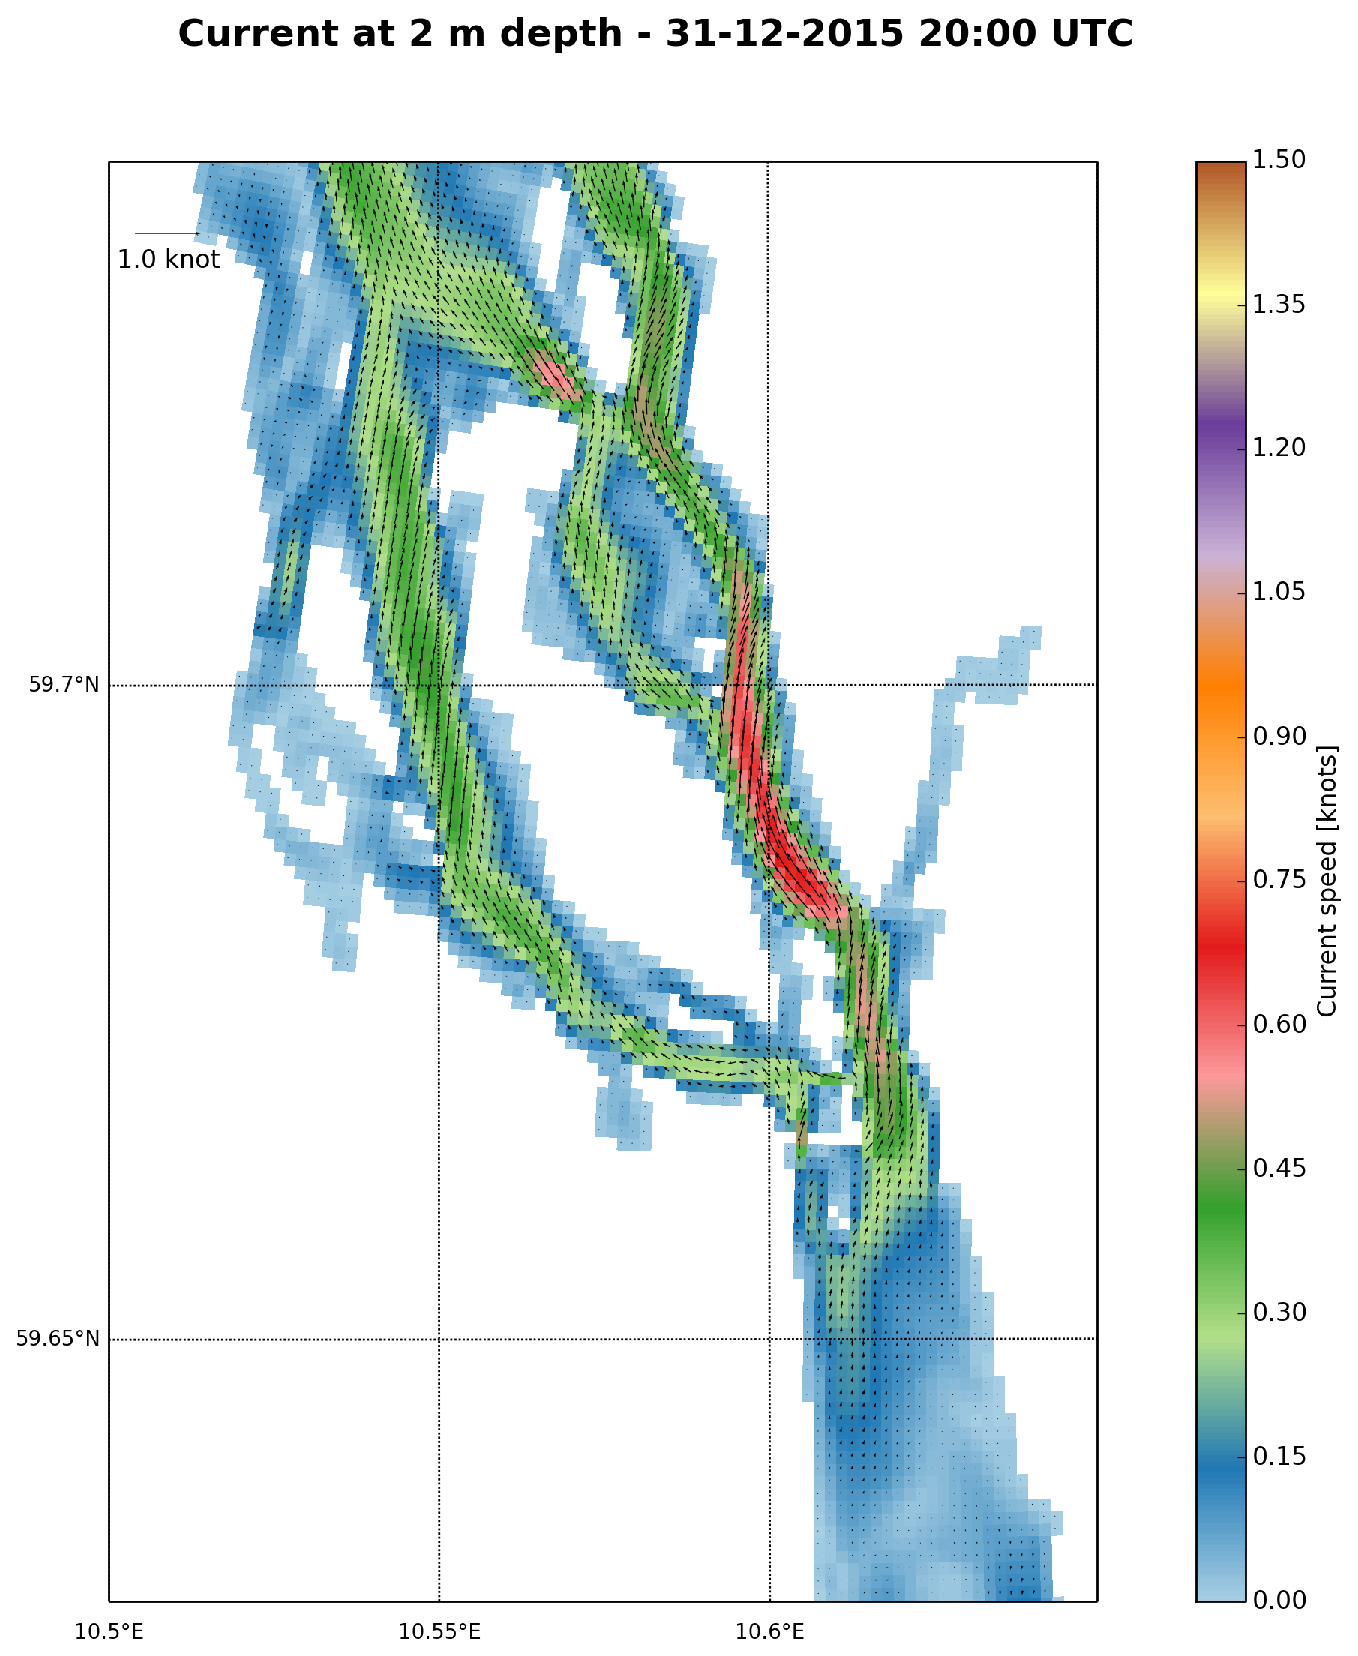
\includegraphics[height=12cm]{droebak__56_current}}
  \end{pspicture}
  \caption{\small  As Figure \ref{fig:indre}, but for the Droebak area.  }
  \label{fig:droebak}
\end{figure}


%%%%%%%%%%%%%%%%%%% Figure 17 Currents in the Drøbak area %%%%%%%%%%%%%%%
\begin{figure}[t]
 \begin{center}
  \begin{pspicture}(0,0)(15,10)
% Include graphs
   \rput[bl]( 0.5,0){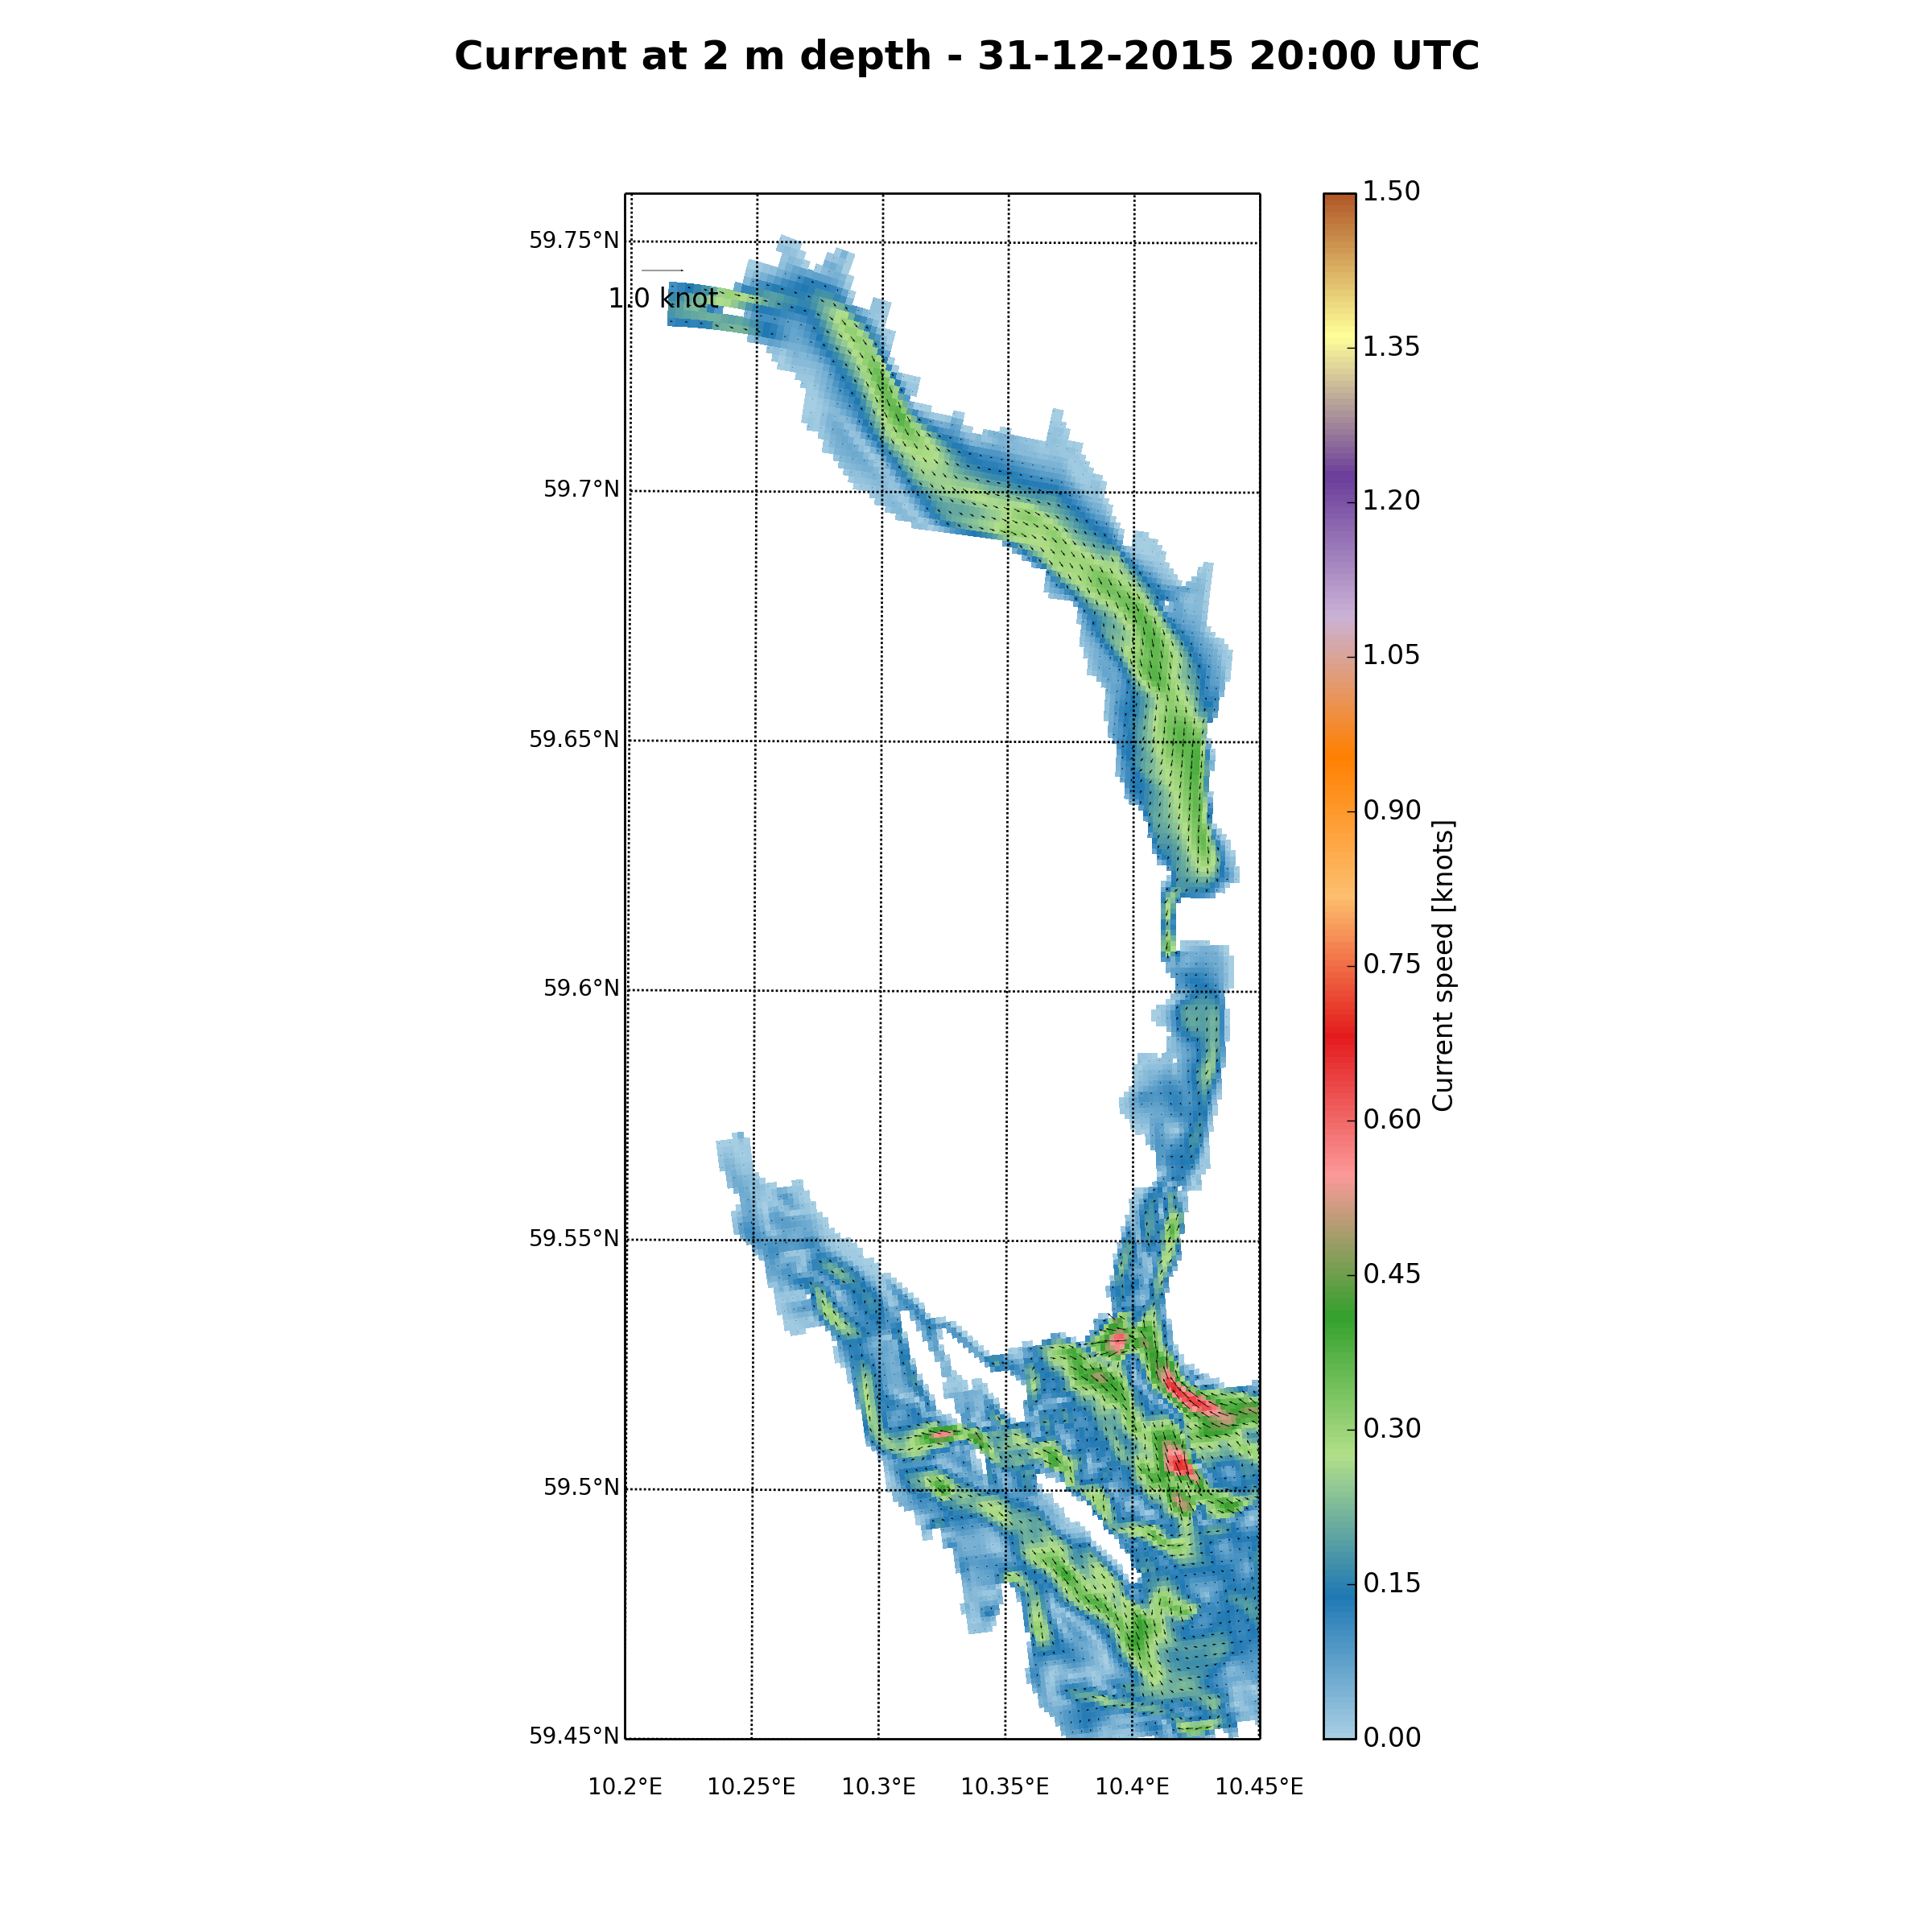
\includegraphics[height=10cm]{drammen1__56_current}}
   \rput[br](15.0,0){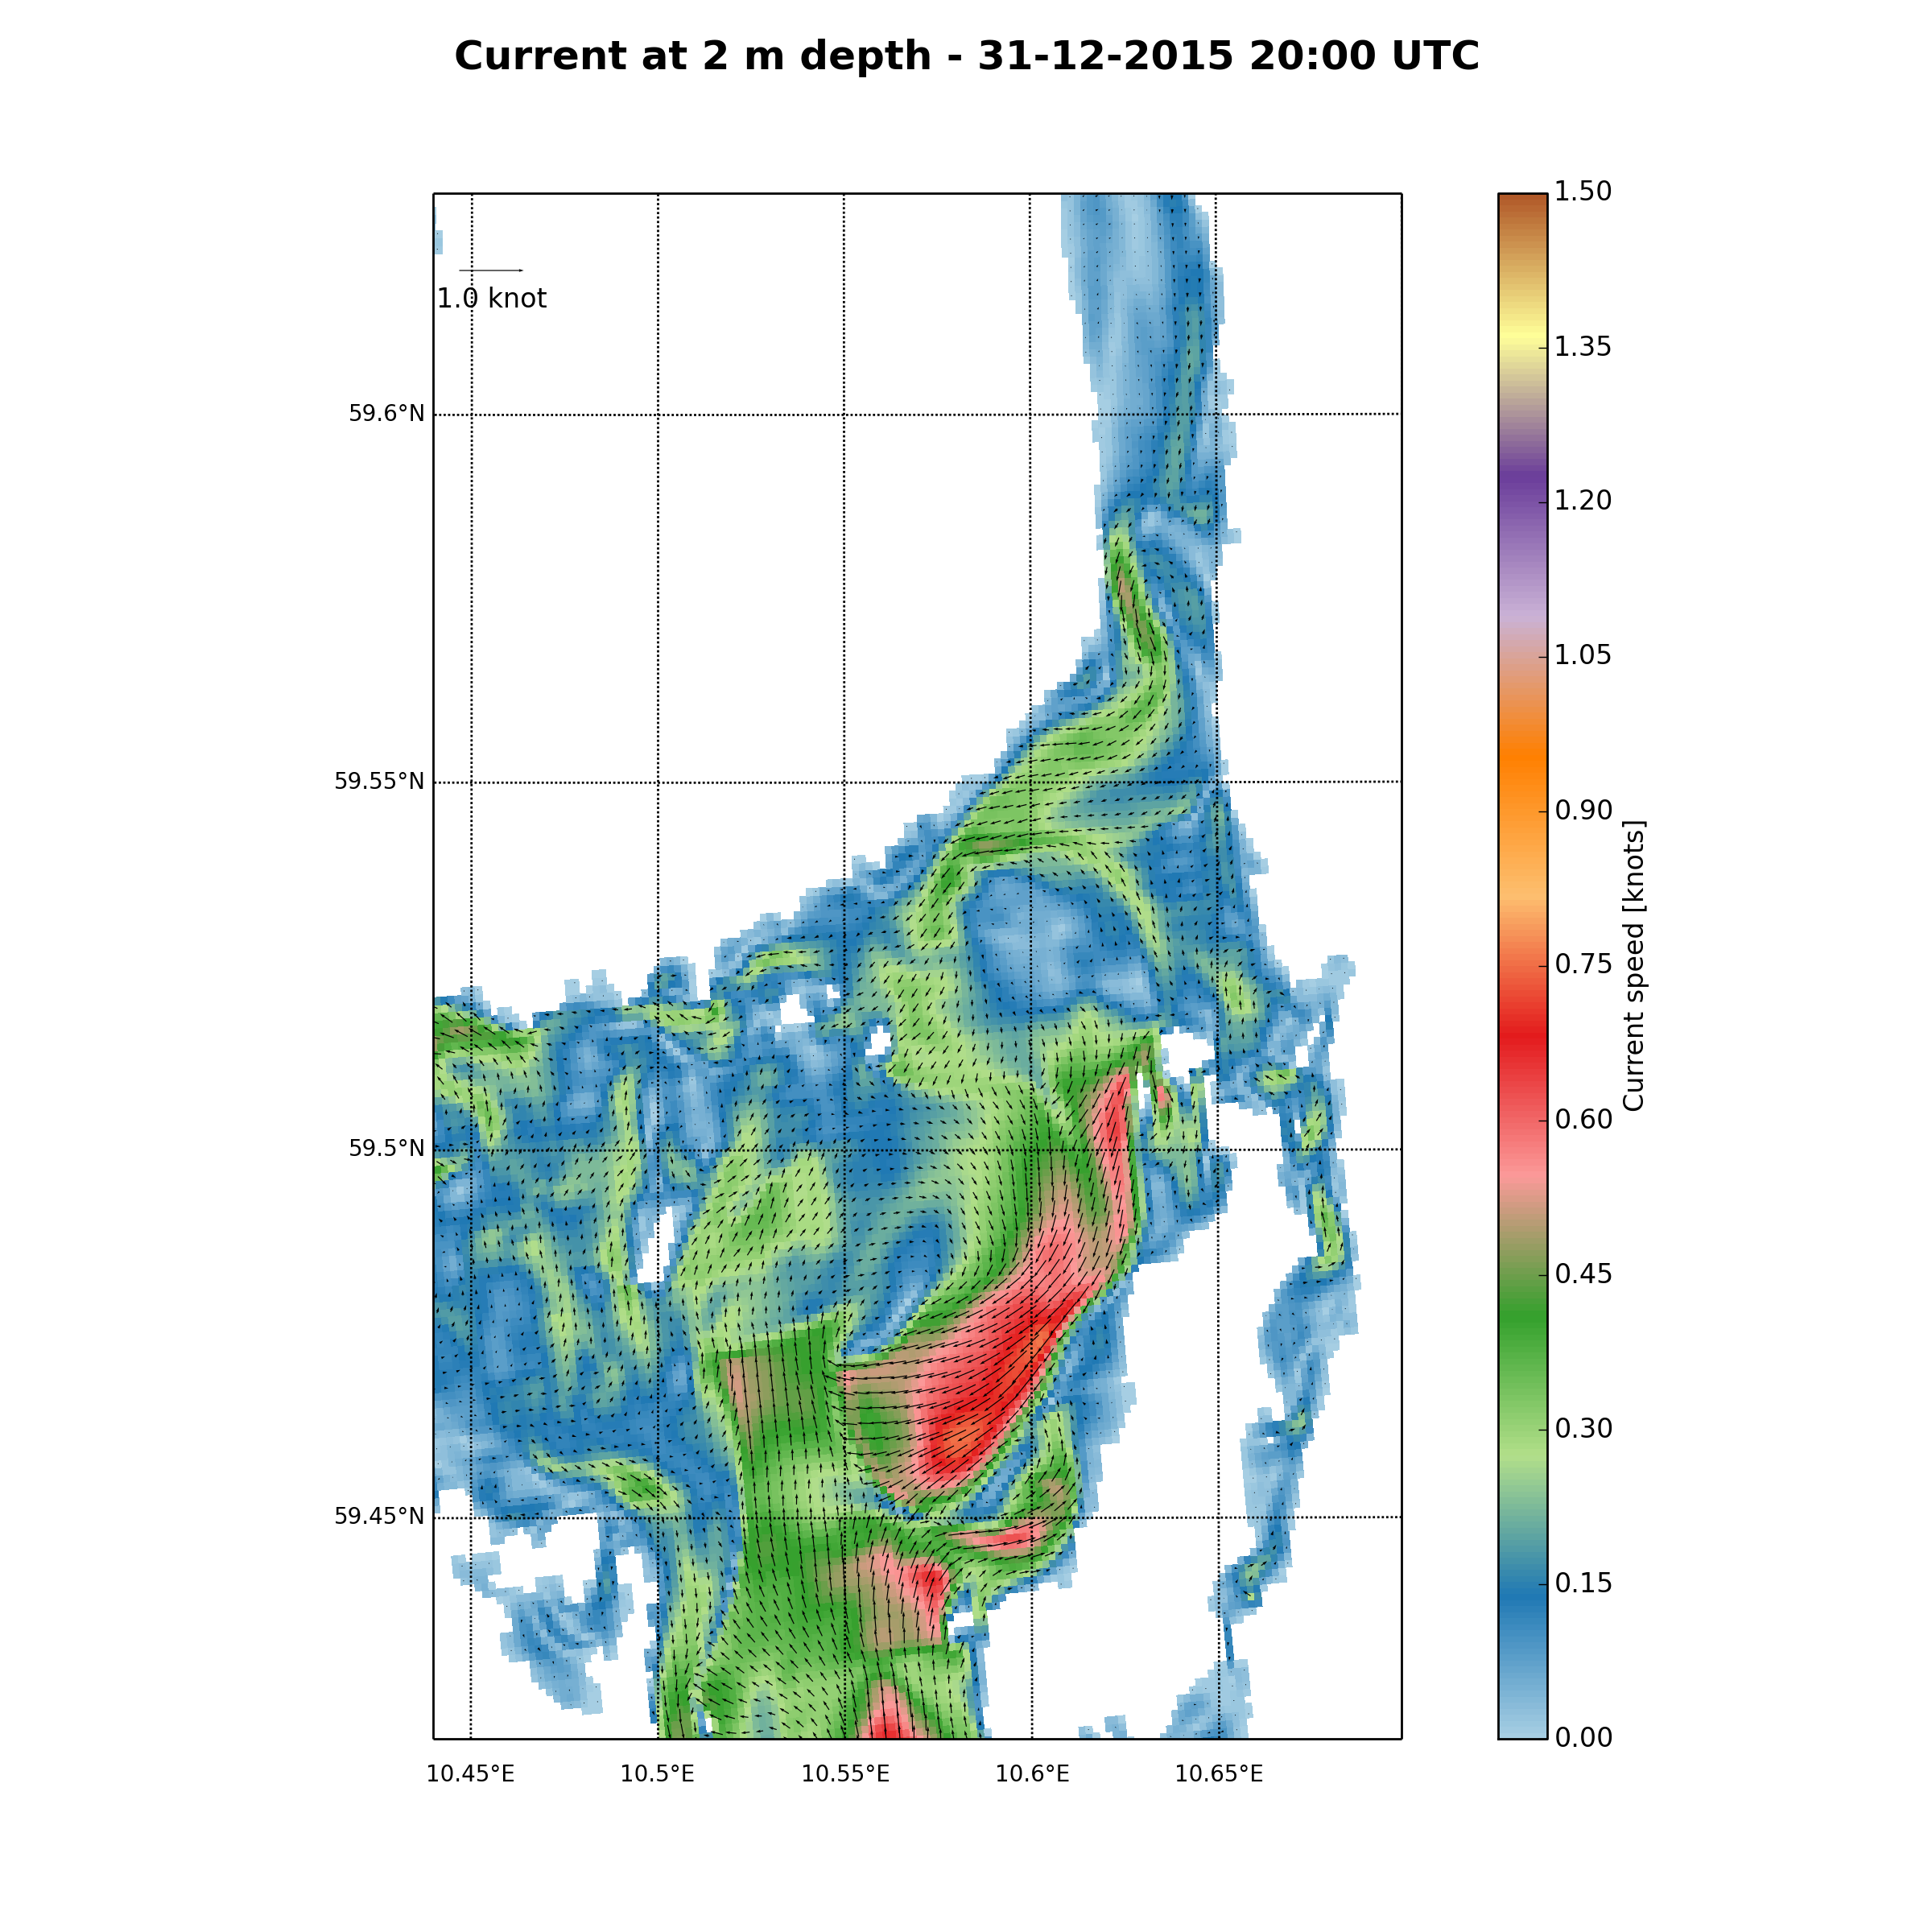
\includegraphics[height=10cm]{breidangen__56_current}}
  \end{pspicture}
  \caption{\small As Figure \ref{fig:indre}, but for the Drammensfjord (left) and Breidangen (right) area.}
  \label{fig:drammen_breidangen}
 \end{center}
\end{figure}


%%%%%%%%%%%%%%%%%%% Figure 17 Currents in the Drøbak area %%%%%%%%%%%%%%%
\begin{figure}[t]
 \begin{center}
  \begin{pspicture}(0,0)(15,19)
% Include graphs
   \rput[b](7.5, 0){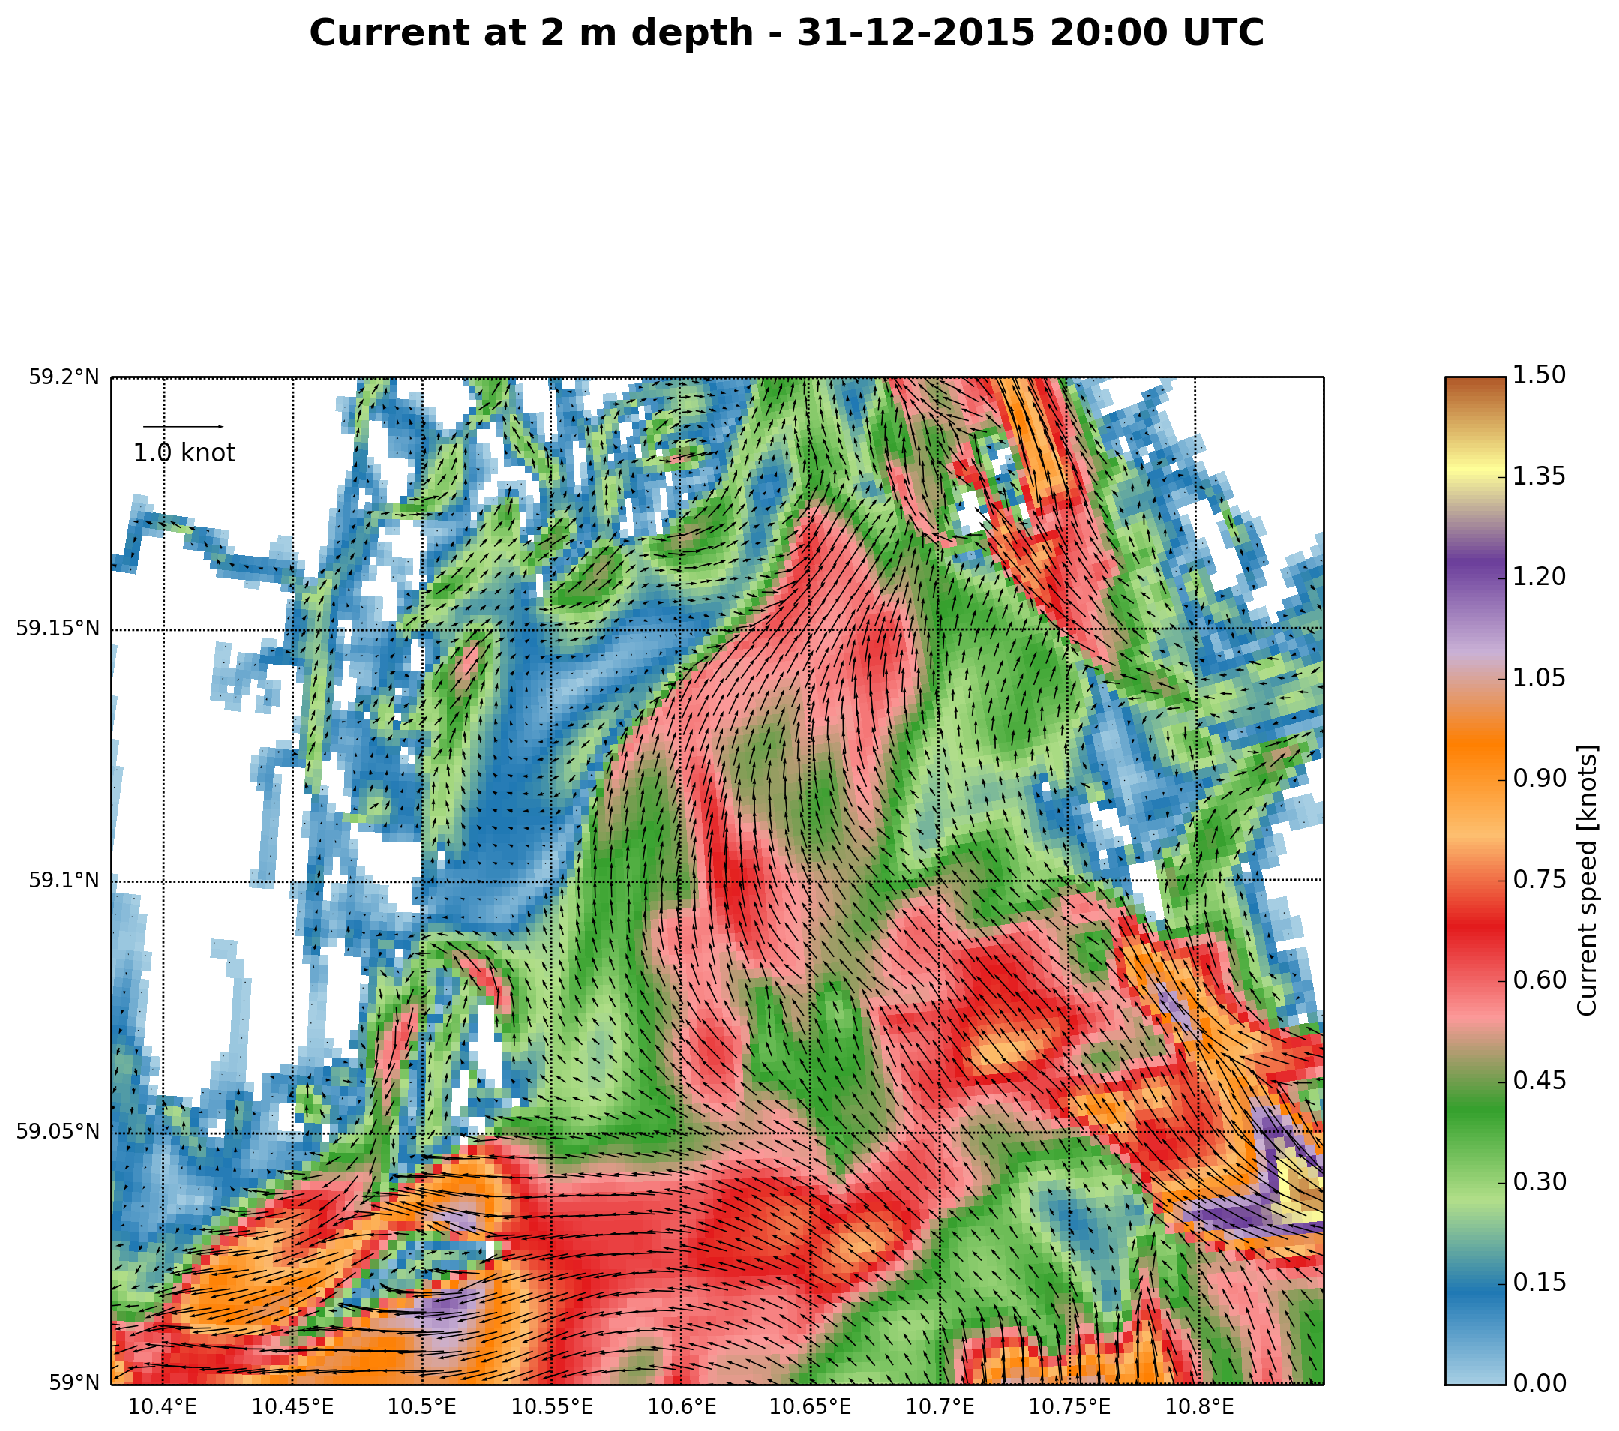
\includegraphics[height=10cm]{tristein__56_current}}
   \rput[b](7.5, 9){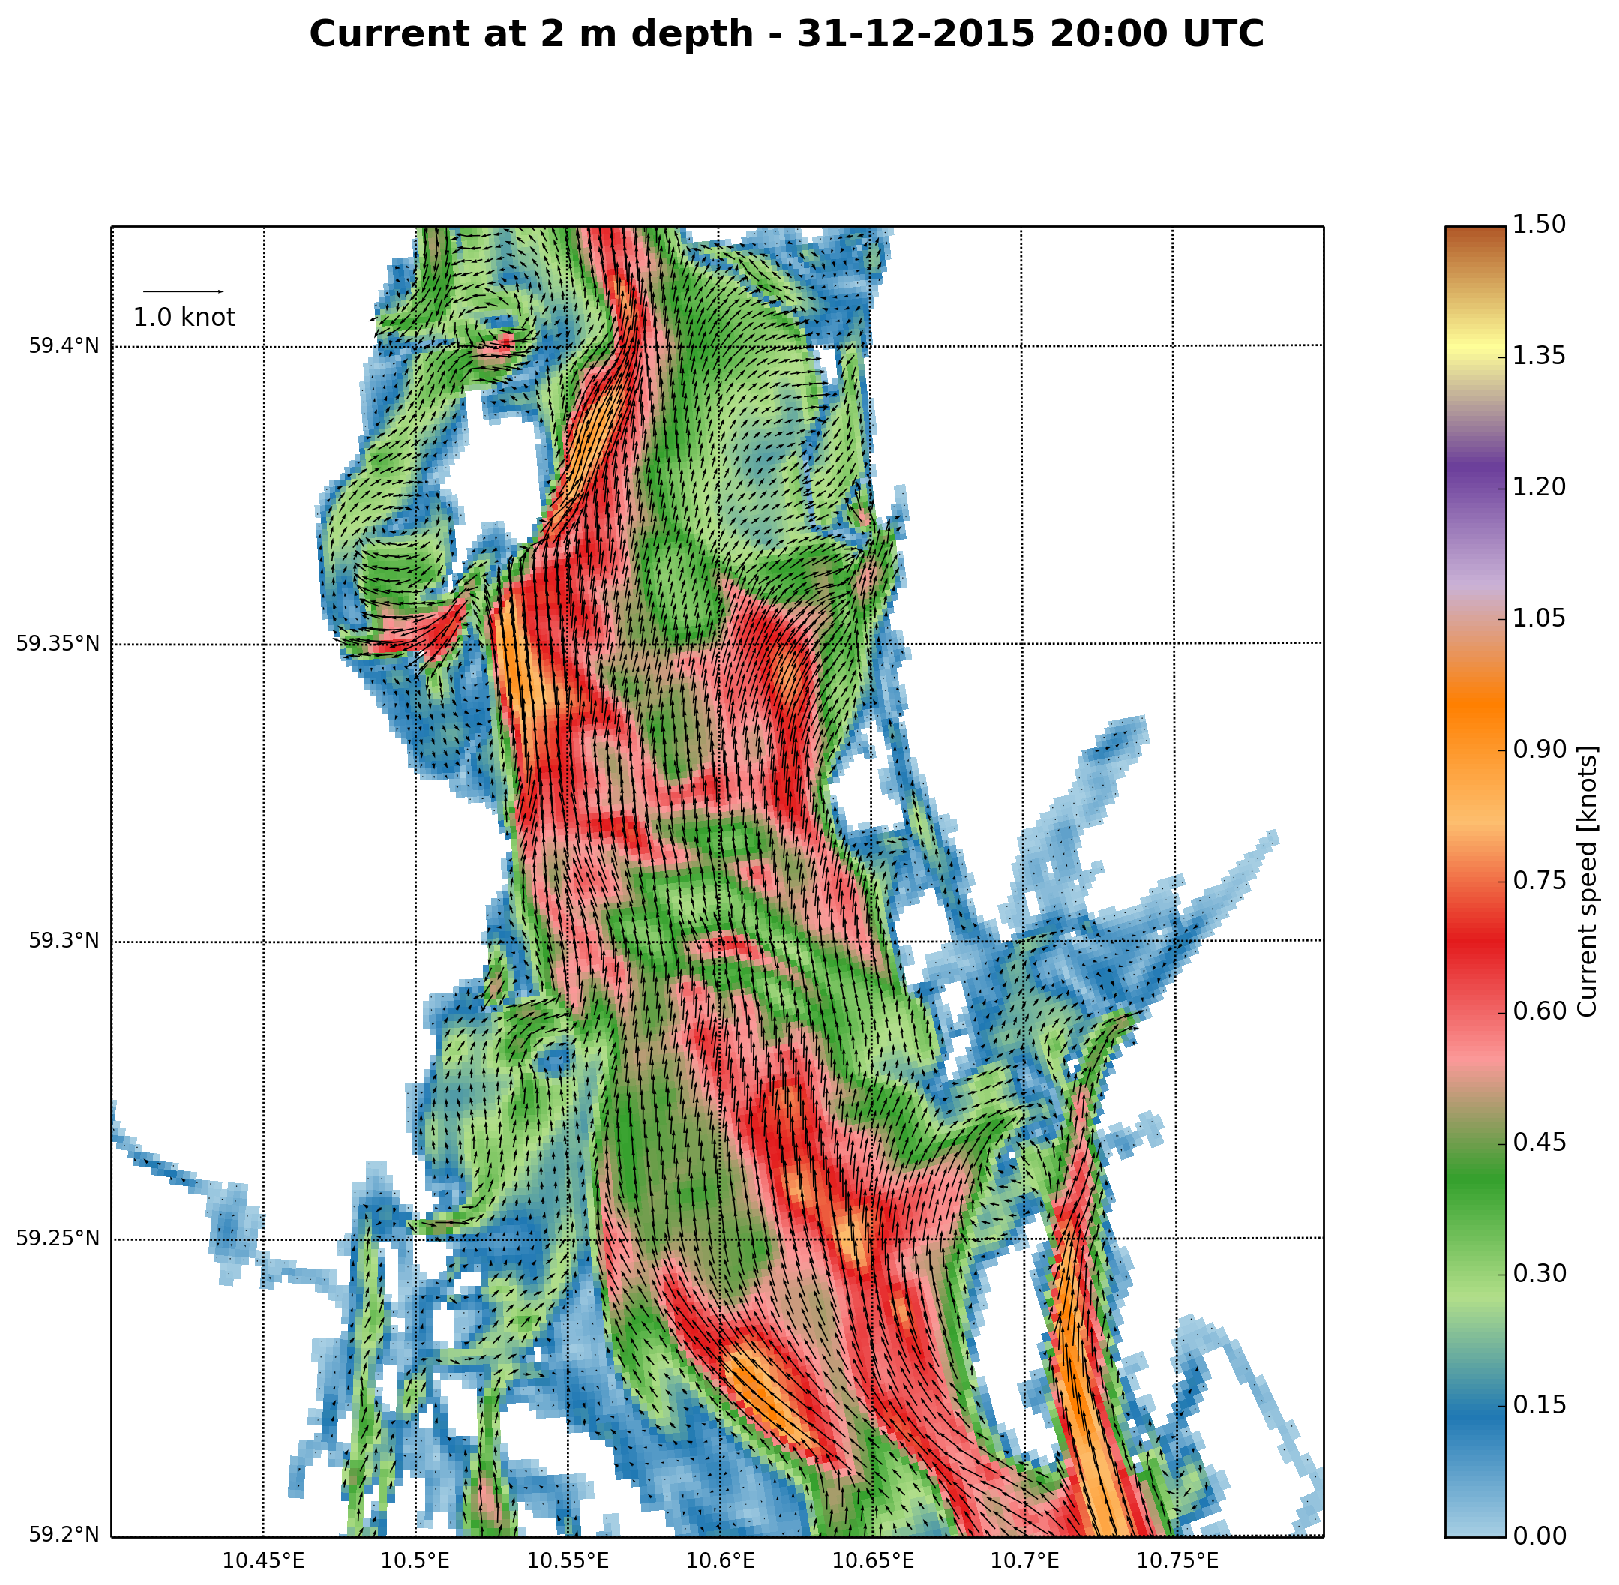
\includegraphics[height=10cm]{slagen__56_current}}
  \end{pspicture}
  \caption{\small As Figure \ref{fig:indre}, but for the Slagen area (top) and Tristein (bottom) area.}
  \label{fig:slagen_tristein}
 \end{center}
\end{figure}



\subsubsection{Temperature}
Figures of interest 

\subsubsection{Salinity}
Figures of interest 

\subsubsection{Sea level}
Figures of interest 



